\documentclass[12pt. a4paper]{report}
\setcounter{secnumdepth}{0} % Turn off section numeration

\usepackage[utf8]{inputenc}
\usepackage[cache=false]{minted}
\usepackage{hyperref}
\usepackage{titlesec}
\usepackage{graphicx}
\graphicspath{ {./images/} }

\titleformat{\chapter}[display]
  {\normalfont\bfseries}{}{0pt}{\Huge}
  

\title{%
	Laboratorul numarul 1 \\
	\large Baze de date}
\author{%
	Dragomir Țurcanu \\
	\large MI-191}
\date{Decembrie 25, 2020}

\begin{document}

\maketitle
\tableofcontents

\chapter{Sarcina}


Deoarece sarcina per-se nu a fost menționată în cadrul aplicației else, o menționez la fel cum este indicată pe website. Deci urmează de realizat însărcinarea în următorul mod.

\begin{quote}
PREZENTAREA VARIANTEI FINALE A APLICAȚIEI WEB, COMPONENTA FRONT-END SI BACK-END, PASII 1-7 CE URMA SA FIE PREZENTAT LA LABORATORUL PRECEDENT
\end{quote}

\section{Obiecivele}

\begin{itemize}
	\item Raportul PDF
	\item Prezentarea PPTX
	\item Prezentarea și zip-ul bazei de date
\end{itemize}

\section{Abordarea Proprie}
Pentru a \emph{simplifica} și în același moment de a \emph{dezvolta} ideea sarcinii, am decis să i-au ca bază laboratorul nr 6 la obiectul "Tehnologii Web", deoarece toate conceptele necesare, ba chiar mai multe sunt folosite și explicate.

Deci am mfoodificat un pic sarcina, pentru a satisface condiția. Varianta lucrării la TW, presupunea crearea unei aplicații de monitorizare și selectare a datelor referitoare la cursul valutar. Și sună în următorul mod.

\begin{quote}
De creat baza de date cu datele despre cursurile valutelor pe fiecare zi. De realizat interfaţa on-line la baza
de date cu următoarele funcţii: selectarea şi vizualizarea datelor în baza cîmpurilor diferite (denumire, data,
perioada de timp), indicarea creşterii sau scăderii cursului în perioada perioadă indicată de utilizator.
\end{quote}

\chapter{Rezolvarea}
Pentru a realiza sarcina, am decis să folosesc un set de tehnologii ce mi-ar fi interesante în lucru, și benefice pentru dezvoltarea skill-setului. De asemenea acestea au contribuit imens le menținerea interesului în dezvoltare :).

\section{Stack-ul Tehnic}
\begin{itemize}
	\item PHP 7.4
	\item MySQL 5.6
	\item Slim Framework \footnote{\url{https://www.slimframework.com/}}
	\item Doctrine ORM \footnote{\url{https://www.doctrine-project.org/projects/orm.html}}
	\item Git \footnote{\url{https://git-scm.com/}}
\end{itemize}

Apropos de Git, proiectul este disponibil deschis pe pagina mea proprie GitHub, pentru citire integrală și instrucțiuni de instalare. Accesați \href{https://github.com/dragomirt/lab6tw}{aici}, sau pe url-ul \url{https://github.com/dragomirt/lab6tw}.

\section{Concepția}
Ideea aplicației este crearea unei interfețe interactive pentru vizualizarea informației. Deoarece caracterul acestei informații este 
\emph{dinamic}, este logică folosirea tehnologiei \textbf{AJAX} \footnote{Asynchronous Javascript and XML}. 

Ținând acest fapt în considerare, am creat o singur loc de intrare, fișierul \textbf{index.html}, ce și conține toată partea vizuală, informația fiind încărcată prin requesturile \textbf{fetch} realizate de către client, pentru a trage informația din \textbf{endpointur-ile} ale \textbf{API-ului} \footnote{Application Programming Interface} intern.

Supranumitul API conține adrese pentru inserarea, modificarea, selectarea și ștergerea informației.

\section{Explicații Tehnice}
Așa deci, odată ce am discutat teoria, este timpul de a demonstra un pic de practică \emph{as well}. Mai jos este demonstrată aplicația în starea sa normală, pe unica pagină grafică a websiteului :D

\begin{figure}
\centering
	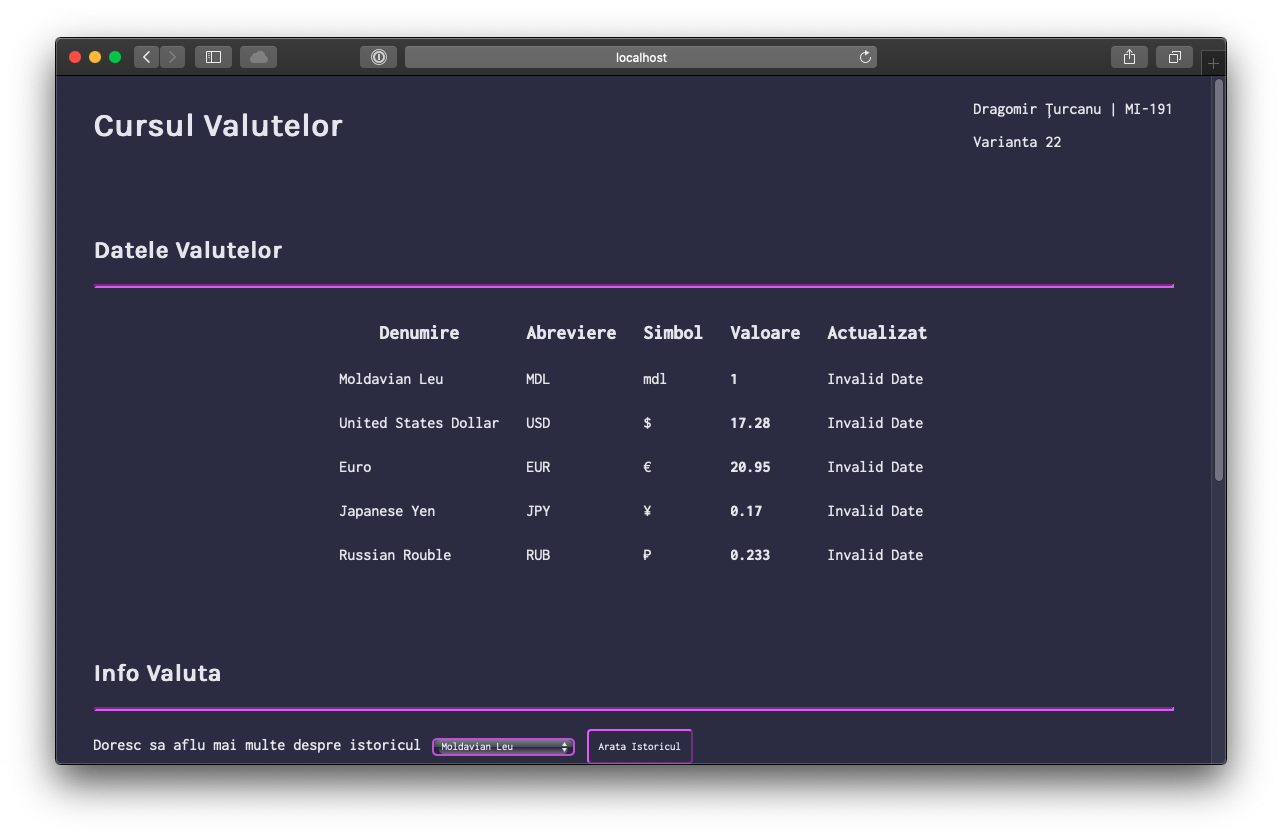
\includegraphics[width=1.0\textwidth]{homepage}
\end{figure}



\definecolor{bg}{rgb}{0.95,0.95,0.95}
\begin{minted}[bgcolor=bg]{php}
<?php
print_f("test", true);
?>
\end{minted}



\end{document}